\chapter{Introduction}\label{ch:introduction}
Around $200,000$ years ago, modern humans evolved in Africa.
Around $120,000-160,000$ years after this, humans migrated out of Africa into
Eurasia~\cite{campbellEvolutionHumanGenetic2010}.
In addition to this, modern humans have interbred with other \textit{Homo sapiens}: Neanderthals and
Denisovans~\cite{sankararamanCombinedLandscapeDenisovan2016}.
The main questions left to answer about the evolutionary history of modern humans are:
``How big was each population at time $t$?''
``Can we get a more accurate date for the migration out of Africa?''
``Are there more species we have admixture with?''
And the overarching question: ``What is the complete demographic model for modern humans?''
\begin{figure}[th]
    \centering{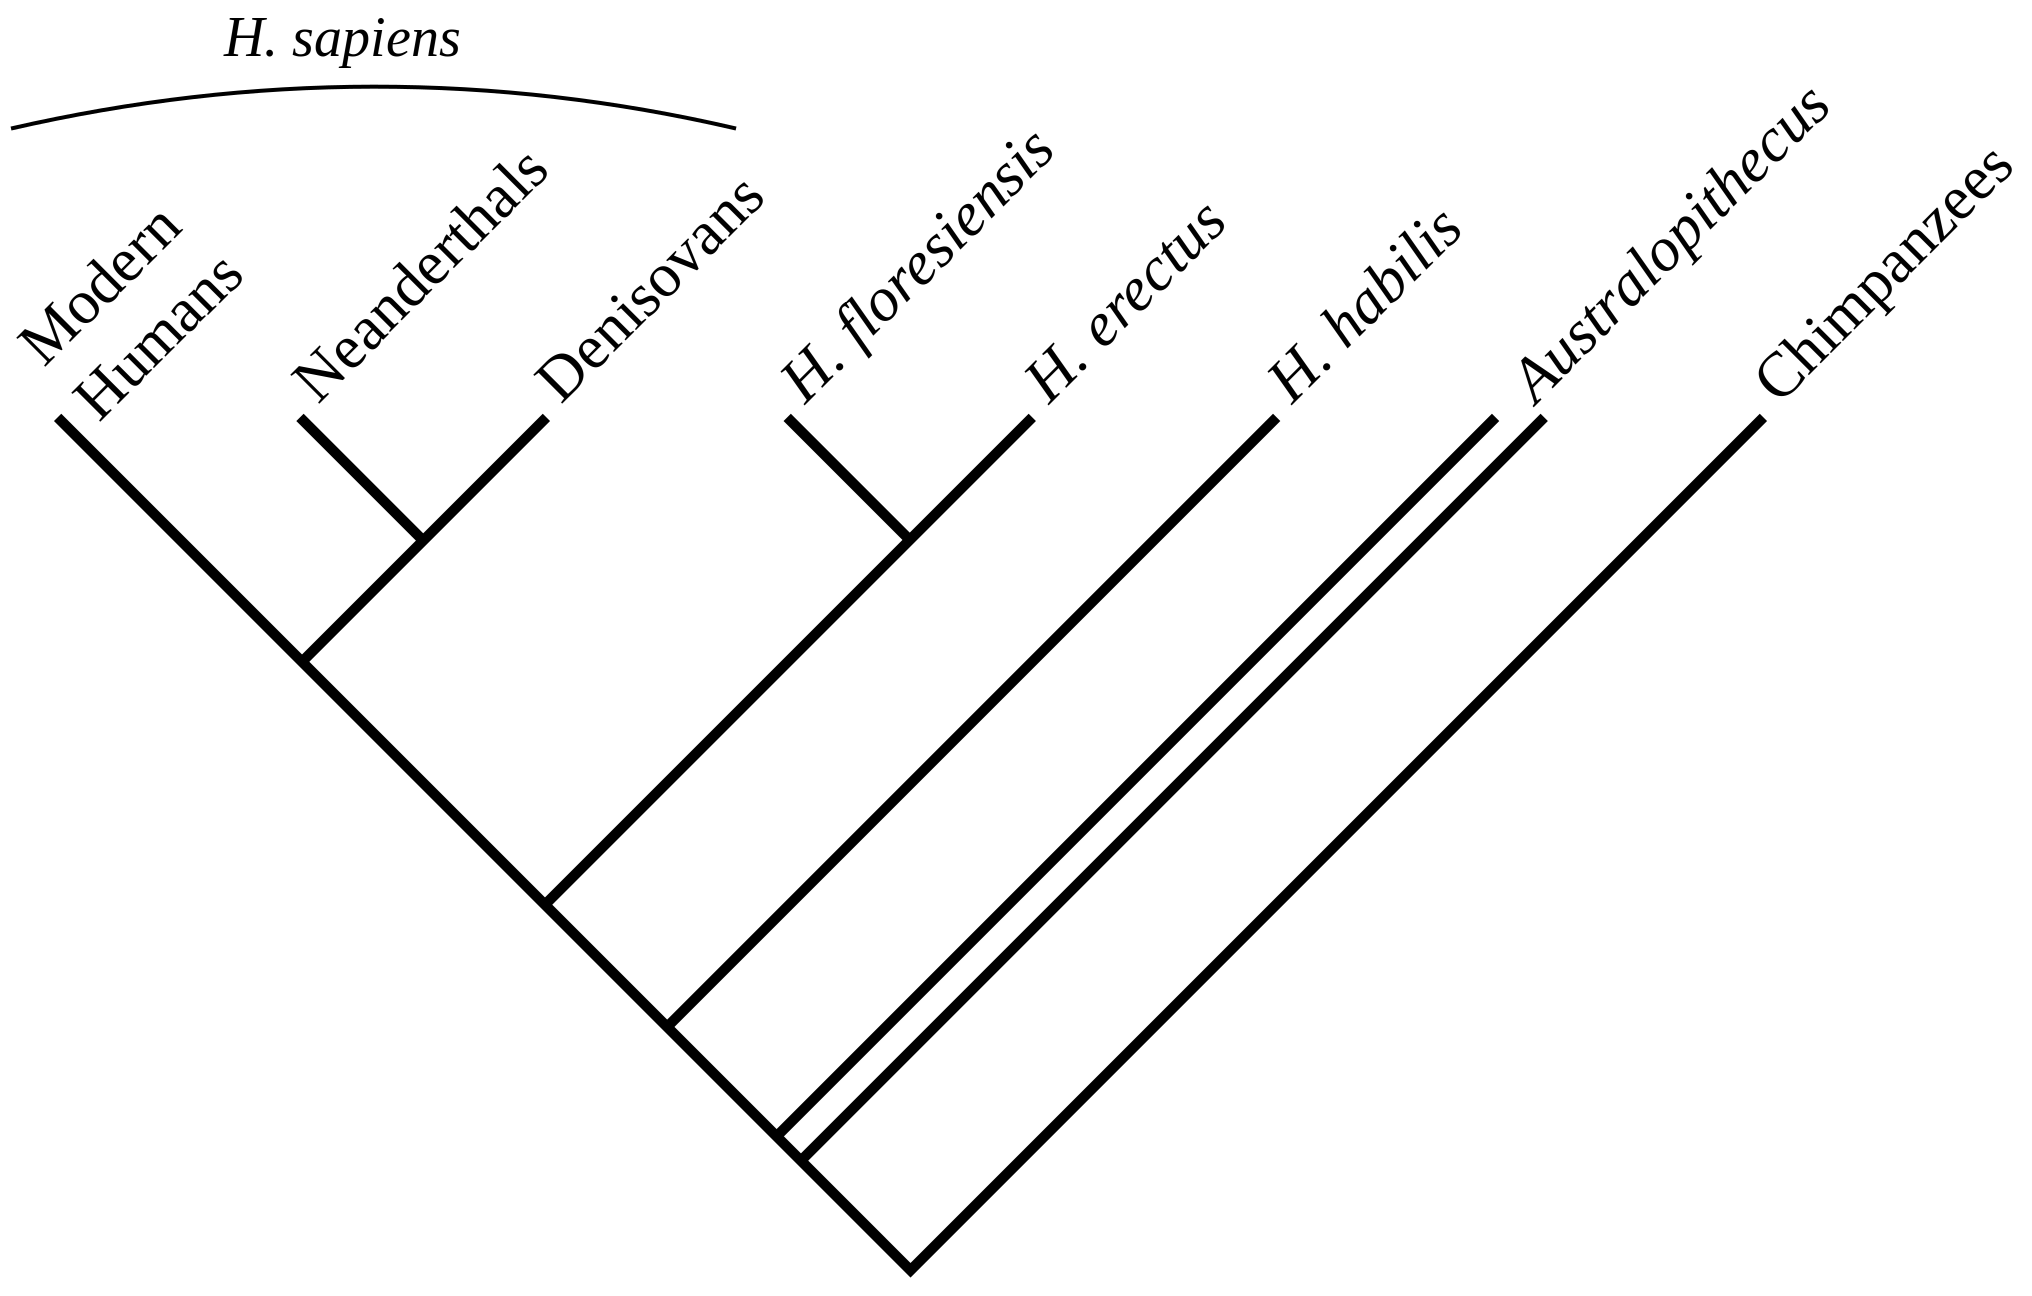
\includegraphics[scale=0.15]{include/images/overview-evolution.png}}
    \caption{
    Phylogeny tree of humans and related species~\cite{riceReview18Organic}.
    }\label{fig:overviewEvolution}
\end{figure}

Where did we get our current estimates?
The answer (for the majority) is genetic variation.
We can infer evolutionary history by tracking how DNA sequences vary (or mutate) from generation to generation.
This is done by constructing different demographic models, and determining the likelihood of said models.
This paper addresses the first step toward being able to do so: finding a reasonable evolutionary model for a
\emph{single} population.

The rest of this paper is organized as follows:
In~\autoref{ch:SNPvsMicrosatellites}, we describe the two most common measures of genetic variation.
In~\autoref{ch:simulatingEvolution}, we describe how to efficiently simulate a microsatellite sample from a coalescing
population.
In~\autoref{ch:modelingMutation}, we discuss how we model microsatellite mutation.
In~\autoref{ch:dataForParameterEstimation}, we briefly describe our observed data.
In~\autoref{ch:parameterEstimation}, we discuss our methods for maximum likelihood estimation.
In~\autoref{ch:discussion}, we describe our methodology and results.
In~\autoref{ch:futureWork}, we discuss what we plan to do after this project.
